\documentclass{article}
\usepackage[utf8]{inputenc}
\usepackage{amssymb}
\usepackage{amsmath}
\usepackage{amsfonts}
\usepackage{mathtools}
\usepackage{hyperref}
\usepackage{fancyhdr, lipsum}
\usepackage{ulem}
\usepackage{fontspec}
\usepackage{xeCJK}
\setCJKmainfont[Path = /usr/share/fonts/TTF/]{edukai-5.0.ttf}
\usepackage{physics}
% \setCJKmainfont{AR PL KaitiM Big5}
% \setmainfont{Times New Roman}
\usepackage{multicol}
\usepackage{zhnumber}
% \usepackage[a4paper, total={6in, 8in}]{geometry}
\usepackage[
	a4paper,
	top=2cm, 
	bottom=2cm,
	left=2cm,
	right=2cm,
	includehead, includefoot,
	heightrounded
]{geometry}
% \usepackage{geometry}
\usepackage{graphicx}
\usepackage{xltxtra}
\usepackage{biblatex} % 引用
\usepackage{caption} % 調整caption位置: \captionsetup{width = .x \linewidth}
\usepackage{subcaption}
% Multiple figures in same horizontal placement
% \begin{figure}[H]
%      \centering
%      \begin{subfigure}[H]{0.4\textwidth}
%          \centering
%          \includegraphics[width=\textwidth]{}
%          \caption{subCaption}
%          \label{fig:my_label}
%      \end{subfigure}
%      \hfill
%      \begin{subfigure}[H]{0.4\textwidth}
%          \centering
%          \includegraphics[width=\textwidth]{}
%          \caption{subCaption}
%          \label{fig:my_label}
%      \end{subfigure}
%         \caption{Caption}
%         \label{fig:my_label}
% \end{figure}
\usepackage{wrapfig}
% Figure beside text
% \begin{wrapfigure}{l}{0.25\textwidth}
%     \includegraphics[width=0.9\linewidth]{overleaf-logo} 
%     \caption{Caption1}
%     \label{fig:wrapfig}
% \end{wrapfigure}
\usepackage{float}
%% 
\usepackage{calligra}
\usepackage{hyperref}
\usepackage{url}
\usepackage{gensymb}
% Citing a website:
% @misc{name,
%   title = {title},
%   howpublished = {\url{website}},
%   note = {}
% }
\usepackage{framed}
% \begin{framed}
%     Text in a box
% \end{framed}
%%

\usepackage{array}
\newcolumntype{F}{>{$}c<{$}} % math-mode version of "c" column type
\newcolumntype{M}{>{$}l<{$}} % math-mode version of "l" column type
\newcolumntype{E}{>{$}r<{$}} % math-mode version of "r" column type
\newcommand{\PreserveBackslash}[1]{\let\temp=\\#1\let\\=\temp}
\newcolumntype{C}[1]{>{\PreserveBackslash\centering}p{#1}} % Centered, length-customizable environment
\newcolumntype{R}[1]{>{\PreserveBackslash\raggedleft}p{#1}} % Left-aligned, length-customizable environment
\newcolumntype{L}[1]{>{\PreserveBackslash\raggedright}p{#1}} % Right-aligned, length-customizable environment

% \begin{center}
% \begin{tabular}{|C{3em}|c|l|}
%     \hline
%     a & b \\
%     \hline
%     c & d \\
%     \hline
% \end{tabular}
% \end{center}    



\usepackage{bm}
% \boldmath{**greek letters**}
\usepackage{tikz}
\usepackage{titlesec}
% standard classes:
% http://tug.ctan.org/macros/latex/contrib/titlesec/titlesec.pdf#subsection.8.2
 % \titleformat{<command>}[<shape>]{<format>}{<label>}{<sep>}{<before-code>}[<after-code>]
% Set title format
% \titleformat{\subsection}{\large\bfseries}{ \arabic{section}.(\alph{subsection})}{1em}{}
\usepackage{amsthm}
\usetikzlibrary{shapes.geometric, arrows}
% https://www.overleaf.com/learn/latex/LaTeX_Graphics_using_TikZ%3A_A_Tutorial_for_Beginners_(Part_3)%E2%80%94Creating_Flowcharts

% \tikzstyle{typename} = [rectangle, rounded corners, minimum width=3cm, minimum height=1cm,text centered, draw=black, fill=red!30]
% \tikzstyle{io} = [trapezium, trapezium left angle=70, trapezium right angle=110, minimum width=3cm, minimum height=1cm, text centered, draw=black, fill=blue!30]
% \tikzstyle{decision} = [diamond, minimum width=3cm, minimum height=1cm, text centered, draw=black, fill=green!30]
% \tikzstyle{arrow} = [thick,->,>=stealth]

% \begin{tikzpicture}[node distance = 2cm]

% \node (name) [type, position] {text};
% \node (in1) [io, below of=start, yshift = -0.5cm] {Input};

% draw (node1) -- (node2)
% \draw (node1) -- \node[adjustpos]{text} (node2);

% \end{tikzpicture}

%%

\DeclareMathAlphabet{\mathcalligra}{T1}{calligra}{m}{n}
\DeclareFontShape{T1}{calligra}{m}{n}{<->s*[2.2]callig15}{}

% Defining a command
% \newcommand{**name**}[**number of parameters**]{**\command{#the parameter number}*}
% Ex: \newcommand{\kv}[1]{\ket{\vec{#1}}}
% Ex: \newcommand{\bl}{\boldsymbol{\lambda}}
\newcommand{\scripty}[1]{\ensuremath{\mathcalligra{#1}}}
% \renewcommand{\figurename}{圖}
\newcommand{\sfa}{\text{  } \forall}
\newcommand{\floor}[1]{\lfloor #1 \rfloor}
\newcommand{\ceil}[1]{\lceil #1 \rceil}


%%
%%
% A very large matrix
% \left(
% \begin{array}{ccccc}
% V(0) & 0 & 0 & \hdots & 0\\
% 0 & V(a) & 0 & \hdots & 0\\
% 0 & 0 & V(2a) & \hdots & 0\\
% \vdots & \vdots & \vdots & \ddots & \vdots\\
% 0 & 0 & 0 & \hdots & V(na)
% \end{array}
% \right)
%%

% amsthm font style 
% https://www.overleaf.com/learn/latex/Theorems_and_proofs#Reference_guide

% 
%\theoremstyle{definition}
%\newtheorem{thy}{Theory}[section]
%\newtheorem{thm}{Theorem}[section]
%\newtheorem{ex}{Example}[section]
%\newtheorem{prob}{Problem}[section]
%\newtheorem{lem}{Lemma}[section]
%\newtheorem{dfn}{Definition}[section]
%\newtheorem{rem}{Remark}[section]
%\newtheorem{cor}{Corollary}[section]
%\newtheorem{prop}{Proposition}[section]
%\newtheorem*{clm}{Claim}
%%\theoremstyle{remark}
%\newtheorem*{sol}{Solution}



\theoremstyle{definition}
\newtheorem{thy}{Theory}
\newtheorem{thm}{Theorem}
\newtheorem{ex}{Example}
\newtheorem{prob}{Problem}
\newtheorem{lem}{Lemma}
\newtheorem{dfn}{Definition}
\newtheorem{rem}{Remark}
\newtheorem{cor}{Corollary}
\newtheorem{prop}{Proposition}
\newtheorem*{clm}{Claim}
%\theoremstyle{remark}
\newtheorem*{sol}{Solution}

% Proofs with first line indent
\newenvironment{proofs}[1][\proofname]{%
  \begin{proof}[#1]$ $\par\nobreak\ignorespaces
}{%
  \end{proof}
}
\newenvironment{sols}[1][]{%
  \begin{sol}[#1]$ $\par\nobreak\ignorespaces
}{%
  \end{sol}
}
%%%%
%Lists
%\begin{itemize}
%  \item ... 
%  \item ... 
%\end{itemize}

%Indexed Lists
%\begin{enumerate}
%  \item ...
%  \item ...

%Customize Index
%\begin{enumerate}
%  \item ... 
%  \item[$\blackbox$]
%\end{enumerate}
%%%%
% \usepackage{mathabx}
\usepackage{xfrac}
%\usepackage{faktor}
%% The command \faktor could not run properly in the pc because of the non-existence of the 
%% command \diagup which sould be properly included in the amsmath package. For some reason 
%% that command just didn't work for this pc 
\newcommand*\quot[2]{{^{\textstyle #1}\big/_{\textstyle #2}}}


\makeatletter
\newcommand{\opnorm}{\@ifstar\@opnorms\@opnorm}
\newcommand{\@opnorms}[1]{%
	\left|\mkern-1.5mu\left|\mkern-1.5mu\left|
	#1
	\right|\mkern-1.5mu\right|\mkern-1.5mu\right|
}
\newcommand{\@opnorm}[2][]{%
	\mathopen{#1|\mkern-1.5mu#1|\mkern-1.5mu#1|}
	#2
	\mathclose{#1|\mkern-1.5mu#1|\mkern-1.5mu#1|}
}
\makeatother
% \opnorm{a}        % normal size
% \opnorm[\big]{a}  % slightly larger
% \opnorm[\Bigg]{a} % largest
% \opnorm*{a}       % \left and \right



\linespread{1.5}
\pagestyle{fancy}
\title{普通天文學2024作業二}
\author{B11202041 物理二 $ $ 劉晁泓}
% \date{\today}
\date{March 23, 2024}
\begin{document}
\maketitle
\thispagestyle{fancy}
\renewcommand{\footrulewidth}{0.4pt}
\cfoot{\thepage}
\renewcommand{\headrulewidth}{0.4pt}
\fancyhead[L]{普通天文學2024作業二}

\setlength{\parindent}{0pt}
Note:本作業請使用太陽質量($1.989 \cdot 10^{30}$ kg)為所有質量的單位\\
$M_{\text{sun}} \rightarrow$ 太陽質量\\
$M_{\text{pc}} \rightarrow 10^6$ pc\\
$\text{AU} \rightarrow 1.5 \cdot 10^8$ km

\setlength{\parindent}{20pt}
\begin{enumerate}
	\item[1.] [10分]課上我們提到暗物質佔目前宇宙整體能量約25\%,
		但是有趣的是,
		在我們日常生活或是太陽系中抑或是地球的運行軌道,
		好像沒有感受到暗物質所提供的重力,
		我們可以透過以下計算來了解暗物質在太陽系尺度下所產生的重力效應。\\
		\par 下圖為銀河系中預期的暗物質密度隨著銀河系中心距離的變化,
		太陽系約位於銀河系8 kpc的位置,
		相對應的按物質質量密度約$6 \cdot 10^6$ ($M_{\text{sun}}/\text{kpc}^3$)。
		根據此資訊,
		估算在地球距離太陽半徑(1AU)的球體積裡,
		暗物質所佔的質量為何(以太陽質量為單位)?

		\begin{figure}[h]
			\centering
			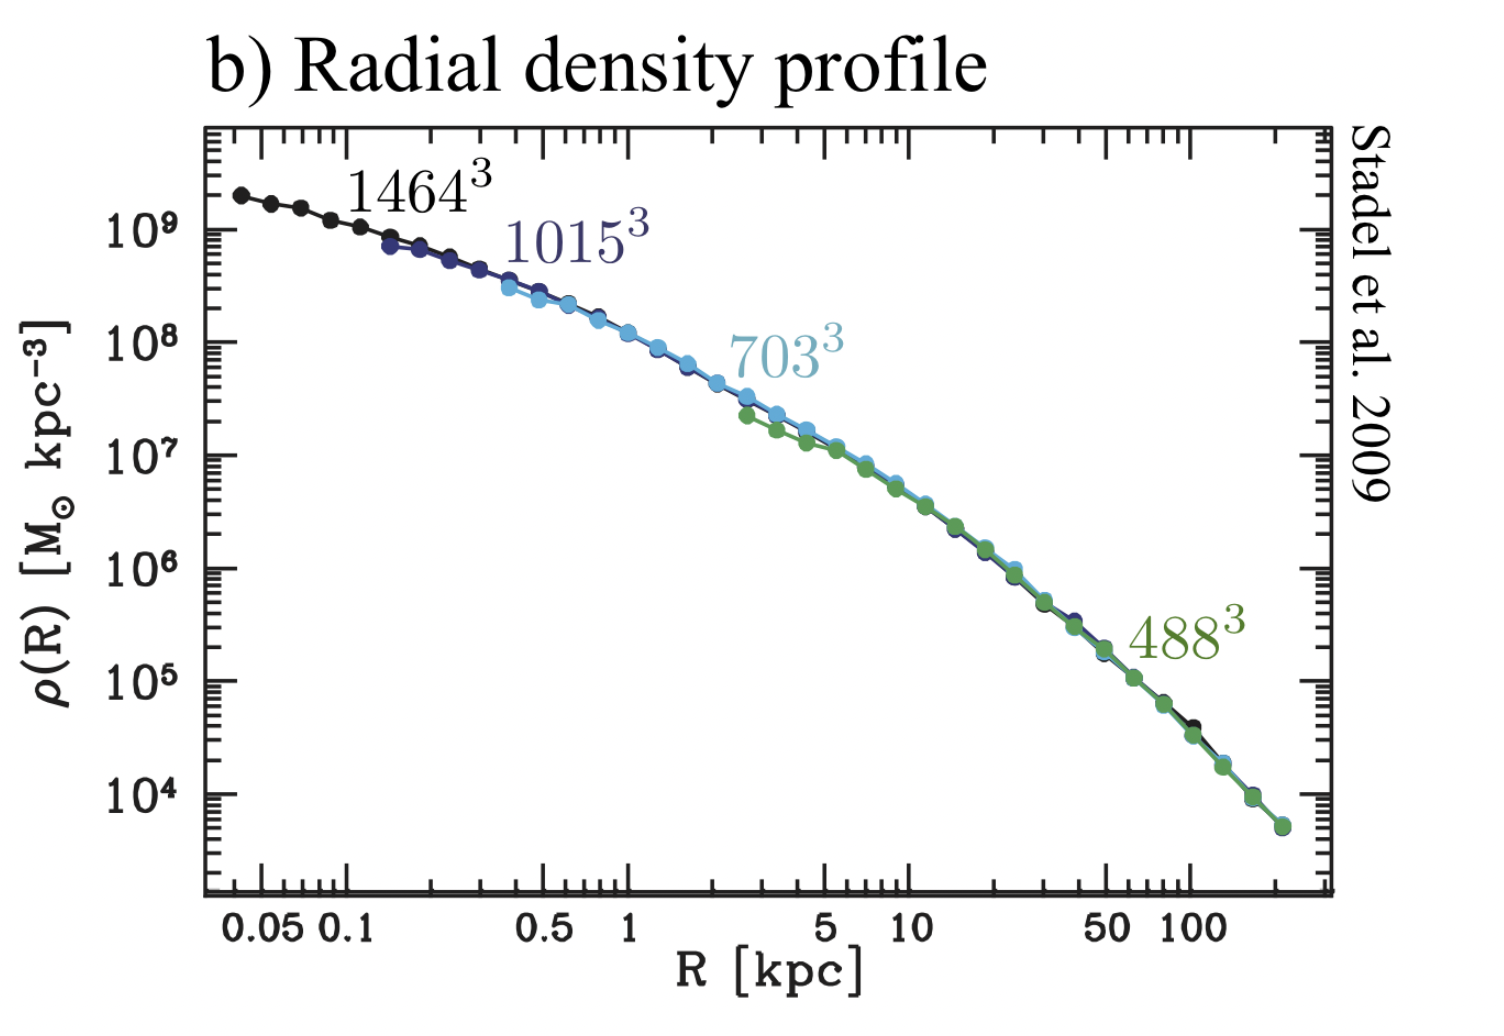
\includegraphics[scale = 0.2]{hw2-1.png}
			\caption{\url{https://arxiv.org/pdf/1404.1938.pdf}}
			\label{fig1}
		\end{figure}

	\item[2.] [10分][圖來自COBE衛星]上課講到COBE衛星觀測CMB,
		將平均值減掉後,
		得到上圖的溫度差,
		根據COBE的結果溫度插為3.3 mK(深紅色是比平均多$\sim 3.3$ mK,
		深藍色是比平均少$\sim 3.3$ mK)。
		根據這個溫度,
		推算出太陽系相對CMB的速度為何?
		[提示如果根據Wien's law,
		溫度變化同等於波長變化,
		波長變化跟速度有關(都普勒效應)]

		\begin{figure}[h]
			\centering
			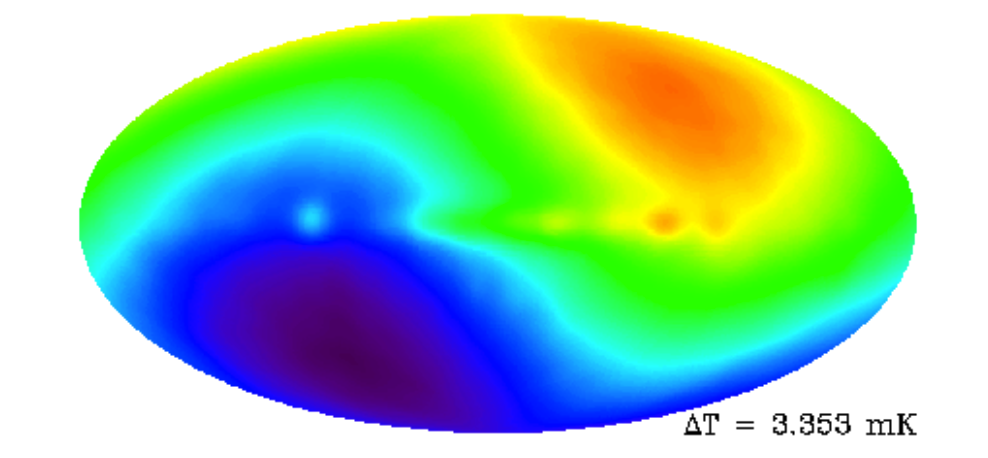
\includegraphics[scale = 0.3]{hw2-2.png}
			\caption{}
			\label{fig2}
		\end{figure}

	\item[3.] [30分]Zwicky當初觀測星系團中的星系的相對速度,
		計算所需要的質量,
		發現暗物質。
		請使用此觀測資料(\href{https://www.dropbox.com/s/6z5jypo7tj2ulen/Virgo_galaxy_catalog.csv?dl=0}{Virgo\_galaxy\_catalog.csv}),
		按照以下步驟做一樣的運算。

		\begin{enumerate}
			\item[(a)] 該數據中有一個"cz"的欄位,
				代表的是那些星系相對太陽系的速度,
				單位km/s。
				請問在該星系團中所有的星系相對太陽系的平均速度為何?

			\item[(b)] cz有一個分佈,
				請問根據數據所計算出來的cz標準差為何?

			\item[(c)] 此標準差值,
				在天文稱為velocity dispersion($\sigma$),
				跟系統內的質量有以下關係($M$為質量)
				\[
					M \simeq \frac{\pi \sigma^2 R}{G}
				\]
				其中$R$是星系團半徑約2 Mpc,
				$G$為重力常數。
				計算該星系團的質量。

			\item[(d)] 該數據中有一個"zmag"的欄位,
				代表那些星系用SDSS z band filter的觀測興等,
				這個星系團離我們的距離為20 Mpc,
				先計算這些星系的絕對興等。
				接著計算這些星系鄉對於太陽有多量
				(太陽在z band的絕對興等為4.5)。
				假設星系的光度鄉對於太陽的光度,
				約等於星系的質量相對於太陽的質量
				(天文稱這個為mass to light ratio),
				計算在這個目錄內所有星系的質量加總。
				這個數星星算出來的質量,
				跟用速度算出來的質量差多少?
				[可以使用任何能幫助你做計算的工具(Excel, google sheet, python, matlab)等等]
				請附上你所使用的程式碼截圖。
				[資料來源:\href{https://ui.adsabs.harvard.edu/abs/2015yCat..22150022K/abstract}{資料1}]
		\end{enumerate}

	\item[4.] [20分]根據宇宙大霹靂理論,
		宇宙年齡約38萬年的時候,
		溫度下降到3000 K,
		光子無法將電子從中性氫中游離開來,
		
		\begin{enumerate}
			\item[(a)] 將電子完全從氫氣游離的能量為13.6 eV,
				試問相對應的光子波長為何?

			\item[(b)] 根據黑體輻射Wien's law,
				該光子波長相對應的溫度又是如何?

			\item[(c)] 請解釋為何不是當宇宙下降到13.6 eV相對應的溫度時,
				光子就無法將電子從中性氫中游離開來,
				為何需要下降到3000 K?

		\end{enumerate}

	\item[5.] [15分] 請看這個\href{https://www.youtube.com/watch?v=JmDszPExepc&ab_channel=issiber}{演講}by Adam Riess [\textbf{1 hour!}],
		根據演講內容回答以下問題。

		\begin{enumerate}
			\item[(a)] 聽完這個演講,
				有哪些東西是你上完這前三週的課之後,
				可以聽得懂的?[100字以內]

			\item[(b)] 聽完這個演講,
				有哪些東西是你沒有聽懂的?[100字以內]

			\item[(c)] 演講中提及用標準燭光所計算的哈伯常數,
				可能會造成系統性誤差的原因有哪些?
				那講者是如何用資料來測試可能的系統性誤差?

		\end{enumerate}

	\item[6.] 上課提到透過CMB偵測暴漲的訊號。
		在2014年,
		一組天文團隊叫BICEP2公佈他們偵測到暴漲的訊號,
		請讀以下\href{https://www.youtube.com/watch?v=JmDszPExepc&ab_channel=issiber}{文章}關於他們的研究成果,
		接著請讀\href{https://phys.org/news/2015-02-cosmic-inflation-bicep2-results.html}{此文章},
		並回答以下問題。
		\begin{enumerate}
			
			\item[(a)] 要偵測暴漲的CMB訊號,
				文章中提到要透過一種polarization的訊號,
				請寫出他的名稱。

			\item[(b)] 請問當初BICEP2認為他們有偵測到暴漲的訊號,
				後來發現該訊號是其他東西所造成的,
				請問那個東西是什麼?

			\item[(c)] 讀完這些結果,
				請寫下你的心得[100字以內]。
		\end{enumerate}

	\item[7.] 請閱讀這篇\href{https://calteches.library.caltech.edu/638/2/Men.pdf}{文章}並寫下你的心得[100字以內]。
		[如果以上連結不能用,使用\href{https://www.dropbox.com/s/yggx7xfldi5fefj/prime_focus_cage_men.pdf}{連結2}]

\end{enumerate}















\end{document}






